\section{Introduction}\label{introduction}

\subsection{\texorpdfstring{\textbf{Background of the Study}}{Background of the Study}}\label{background-of-the-study}

\subsubsection{\texorpdfstring{\textbf{What is Real Estate?}}{What is Real Estate?}}\label{what-is-real-estate}

Real estate sits at the intersection of shelter, commerce, and investment. Under Article 415 of the Philippine Civil Code, immovable property includes land, buildings, and permanent attachments. Unlike many other assets, real estate is both something people use and something they price, finance, and trade.

In actual transactions, that price is shaped by several actors with different interests. Brokers and agents facilitate sales, banks finance purchases and assess collateral risk, appraisers estimate value, and local government units set administrative benchmarks such as zonal values for taxation. Although these actors approach property from different functions, all depend on a defensible estimate of value. This study examined how that value is determined, how fair it is, and how transparent the valuation process can be.

\subsubsection{\texorpdfstring{\textbf{Real Estate in Cebu}}{Real Estate in Cebu}}\label{real-estate-in-cebu}

Cebu has become one of the Philippines' most dynamic regional economies, recording 7.3\% growth in 2024 (PSA Region 7, 2025). Much of this growth has come from the IT-BPM sector, the expansion of call center activity, and the post-pandemic recovery of tourism, hospitality, and retail. These shifts have fed directly into demand for residential and mixed-use property.

Across Metro Cebu, particularly Cebu City, Mandaue, Lapu-Lapu, Talisay, Minglanilla, and Consolacion, that demand has made the property market notably active. Residential property prices in the area rose by 11.5\% in 2025, the highest rate outside the National Capital Region (BSP, 2025).

That pressure is also being reinforced by infrastructure projects that are changing accessibility across the urban area. The Cebu Bus Rapid Transit (CBRT), the Metro Cebu Expressway, and the continued development of the South Road Properties are likely to affect land values by altering connectivity, travel times, and the attractiveness of nearby locations. For a valuation study, these spatial shifts matter because they change not only where demand is strongest, but also how quickly existing benchmarks can become outdated.

\subsubsection{\texorpdfstring{\textbf{The Problem: How is Price Decided in Cebu?}}{The Problem: How is Price Decided in Cebu?}}\label{the-problem-how-is-price-decided-in-cebu}

Despite this growth, the property pricing system in Metro Cebu is still assembled from several partial and often inconsistent reference points. In practice, three sources are used most often, and each has clear limitations.

First, BIR zonal values serve as administrative benchmarks for taxation, but they often lag behind actual market conditions. A 2023 appraisal review found that only 60\% of LGUs nationwide had updated their assessment schedules (Otsuka et al., 2023), which suggests that some zonal values in Cebu may no longer reflect current prices. Second, bank appraisals are designed mainly to manage lending risk, so they may produce values that are more conservative than open-market prices. Third, listing prices and agent quotes often reflect asking positions rather than verified transaction values, and these are not standardized across platforms or sellers.

The result is a valuation gap between official benchmarks, estimates based on lenders, and prices that markets are seemingly willing to bear. For buyers and sellers, this makes pricing harder to interpret. For banks, it complicates collateral assessment. For local governments, it weakens the connection between tax benchmarks and market reality. Metro Cebu therefore has an active property market, but not yet a consistent and validated valuation system at the property level.

\subsubsection{\texorpdfstring{\textbf{Why Metro Cebu, and Why Now?}}{Why Metro Cebu, and Why Now?}}\label{why-metro-cebu-and-why-now}

Three converging factors make it timely to build a data-driven valuation model for Metro Cebu:

\begin{enumerate}
\item \textbf{Prices are moving faster than the benchmarks can follow}: With 11.5\% growth in 2025 and some zonal values outdated since 2019, the gap between official benchmarks and market reality is widening. Continued reliance on outdated models perpetuates mispricing.
\item \textbf{Infrastructure is redrawing the value map in real time}: Projects like the CBRT and the Expressway are restructuring barangay accessibility and desirability. Traditional appraisal methods, reliant on historical comparables, cannot price these spatial changes in real time. A GIS-augmented model built on geocoded property data addresses this constraint.
\item \textbf{The data now exists to do this properly}: Online platforms such as Lamudi, open geospatial data, and geocoding tools (Google Maps API) enable the construction of a property-level dataset without requiring private deed-of-sale records. Open-source GIS software also allows us to transform this data into an interactive web map, providing prescriptive spatial decision support for practitioners.
\end{enumerate}

\subsubsection{\texorpdfstring{\textbf{Ideal Scenario}}{Ideal Scenario}}\label{ideal-scenario}

The core problem is not that Cebu lacks valuation activity, but that the activity still lacks a common, evidence-based basis. A data-driven model that quantifies the contribution of specific value drivers, such as lot area, proximity to economic nodes, nearby amenities, and neighborhood trends, would provide reproducible estimates for residential properties. Delivered through an interactive QGIS map and a Streamlit web application, this model would help move Cebu from heuristic pricing toward a more transparent and evidence-based valuation process aligned with IVS 2025.

\begin{center}\rule{0.5\linewidth}{0.5pt}\end{center}

\subsection{\texorpdfstring{\textbf{Statement of the Problem}}{Statement of the Problem}}\label{statement-of-the-problem}

\textbf{Decision Problem}: How can real estate firms in Metro Cebu utilize data-driven models, augmented with geospatial feature engineering, to predict property values more accurately and consistently?

\textbf{Research Problem}: In Metro Cebu, reliance on outdated administrative benchmarks and manual appraisals produces inconsistent, subjective pricing. No existing study combines property-level data with GIS-derived geospatial features (network distance, MCRAI scoring, spatial autocorrelation) for the Metro Cebu market, and none provides a spatial decision-support layer for valuation practice.

\begin{center}\rule{0.5\linewidth}{0.5pt}\end{center}

\subsection{\texorpdfstring{\textbf{Research Questions}}{Research Questions}}\label{research-questions}

\begin{enumerate}
\item What value drivers significantly influence property prices in Metro Cebu?
\item Which modeling technique---\textbf{Hedonic Regression}, \textbf{Random Forest}, or \textbf{XGBoost}---produces the most accurate valuation out of sample (lowest MAPE)?
\item Do \textbf{geospatial features}---proximity to economic nodes, MCRAI accessibility measures, and spatial autocorrelation---significantly improve model performance compared to structural-only models?
\item How large is the ``Valuation Gap'' between the model's data-driven predictions and traditional BIR Zonal Values?
\end{enumerate}

\begin{center}\rule{0.5\linewidth}{0.5pt}\end{center}

\subsection{\texorpdfstring{\textbf{Significance of the Study}}{Significance of the Study}}\label{significance-of-the-study}

Addressing this valuation gap benefits multiple stakeholders:

\begin{enumerate}
\item \textbf{Real Estate Brokers and Appraisers}: Provides standardized tools compliant with IVS 2025 transparency requirements, including SHAP-based explainability, an interactive QGIS map for spatial analysis, and a Streamlit interface for property-level valuation review.
\item \textbf{Property Investors}: Ensures fair, data-backed pricing and helps identify undervalued areas visually through geospatial heatmaps.
\item \textbf{Banks and Lending Institutions}: Improves collateral assessment accuracy through reproducible, auditable models, which reduce exposure to pricing errors that manual appraisals can miss.
\item \textbf{Local Government Units (LGUs)}: Facilitates the updating of zonal values using market-based evidence, mapping the geographic divergence between official and actual prices.
\end{enumerate}

This study is significant within the Philippine context as the first Cebu-specific, data-driven valuation model integrating GIS-based feature engineering. While prior Philippine machine learning studies focus on Metro Manila or use aggregate indices, no work applies geocoded network-distance features, MCRAI scoring, and spatial autocorrelation to property-level data for Metro Cebu. By delivering results through QGIS-ready map layers and a Streamlit web application, the study extends predictive analytics into applied decision support for a fragmented local market.

\begin{center}\rule{0.5\linewidth}{0.5pt}\end{center}

\subsection{\texorpdfstring{\textbf{Scope and Limitations}}{Scope and Limitations}}\label{scope-and-limitations}

\subsubsection{\texorpdfstring{\textbf{Scope}}{Scope}}\label{scope}

This study focuses on the residential real estate market within Metro Cebu. While the National Economic and Development Authority (NEDA) defines Metro Cebu as encompassing 13 LGUs, this study operationally scopes ``Metro Cebu'' to its central urban core: \textbf{Cebu City, Mandaue, Lapu-Lapu, Talisay, Minglanilla, and Consolacion}. This constraint ensures high data density and robust geospatial analysis, as these six LGUs represent the most active transaction zones and the highest concentration of infrastructure development. Figure~\ref{fig:study-area} shows the spatial extent of this scope and the locations of the eight polycentric CBD nodes used in the model.

\begin{figure}[htbp]
\centering
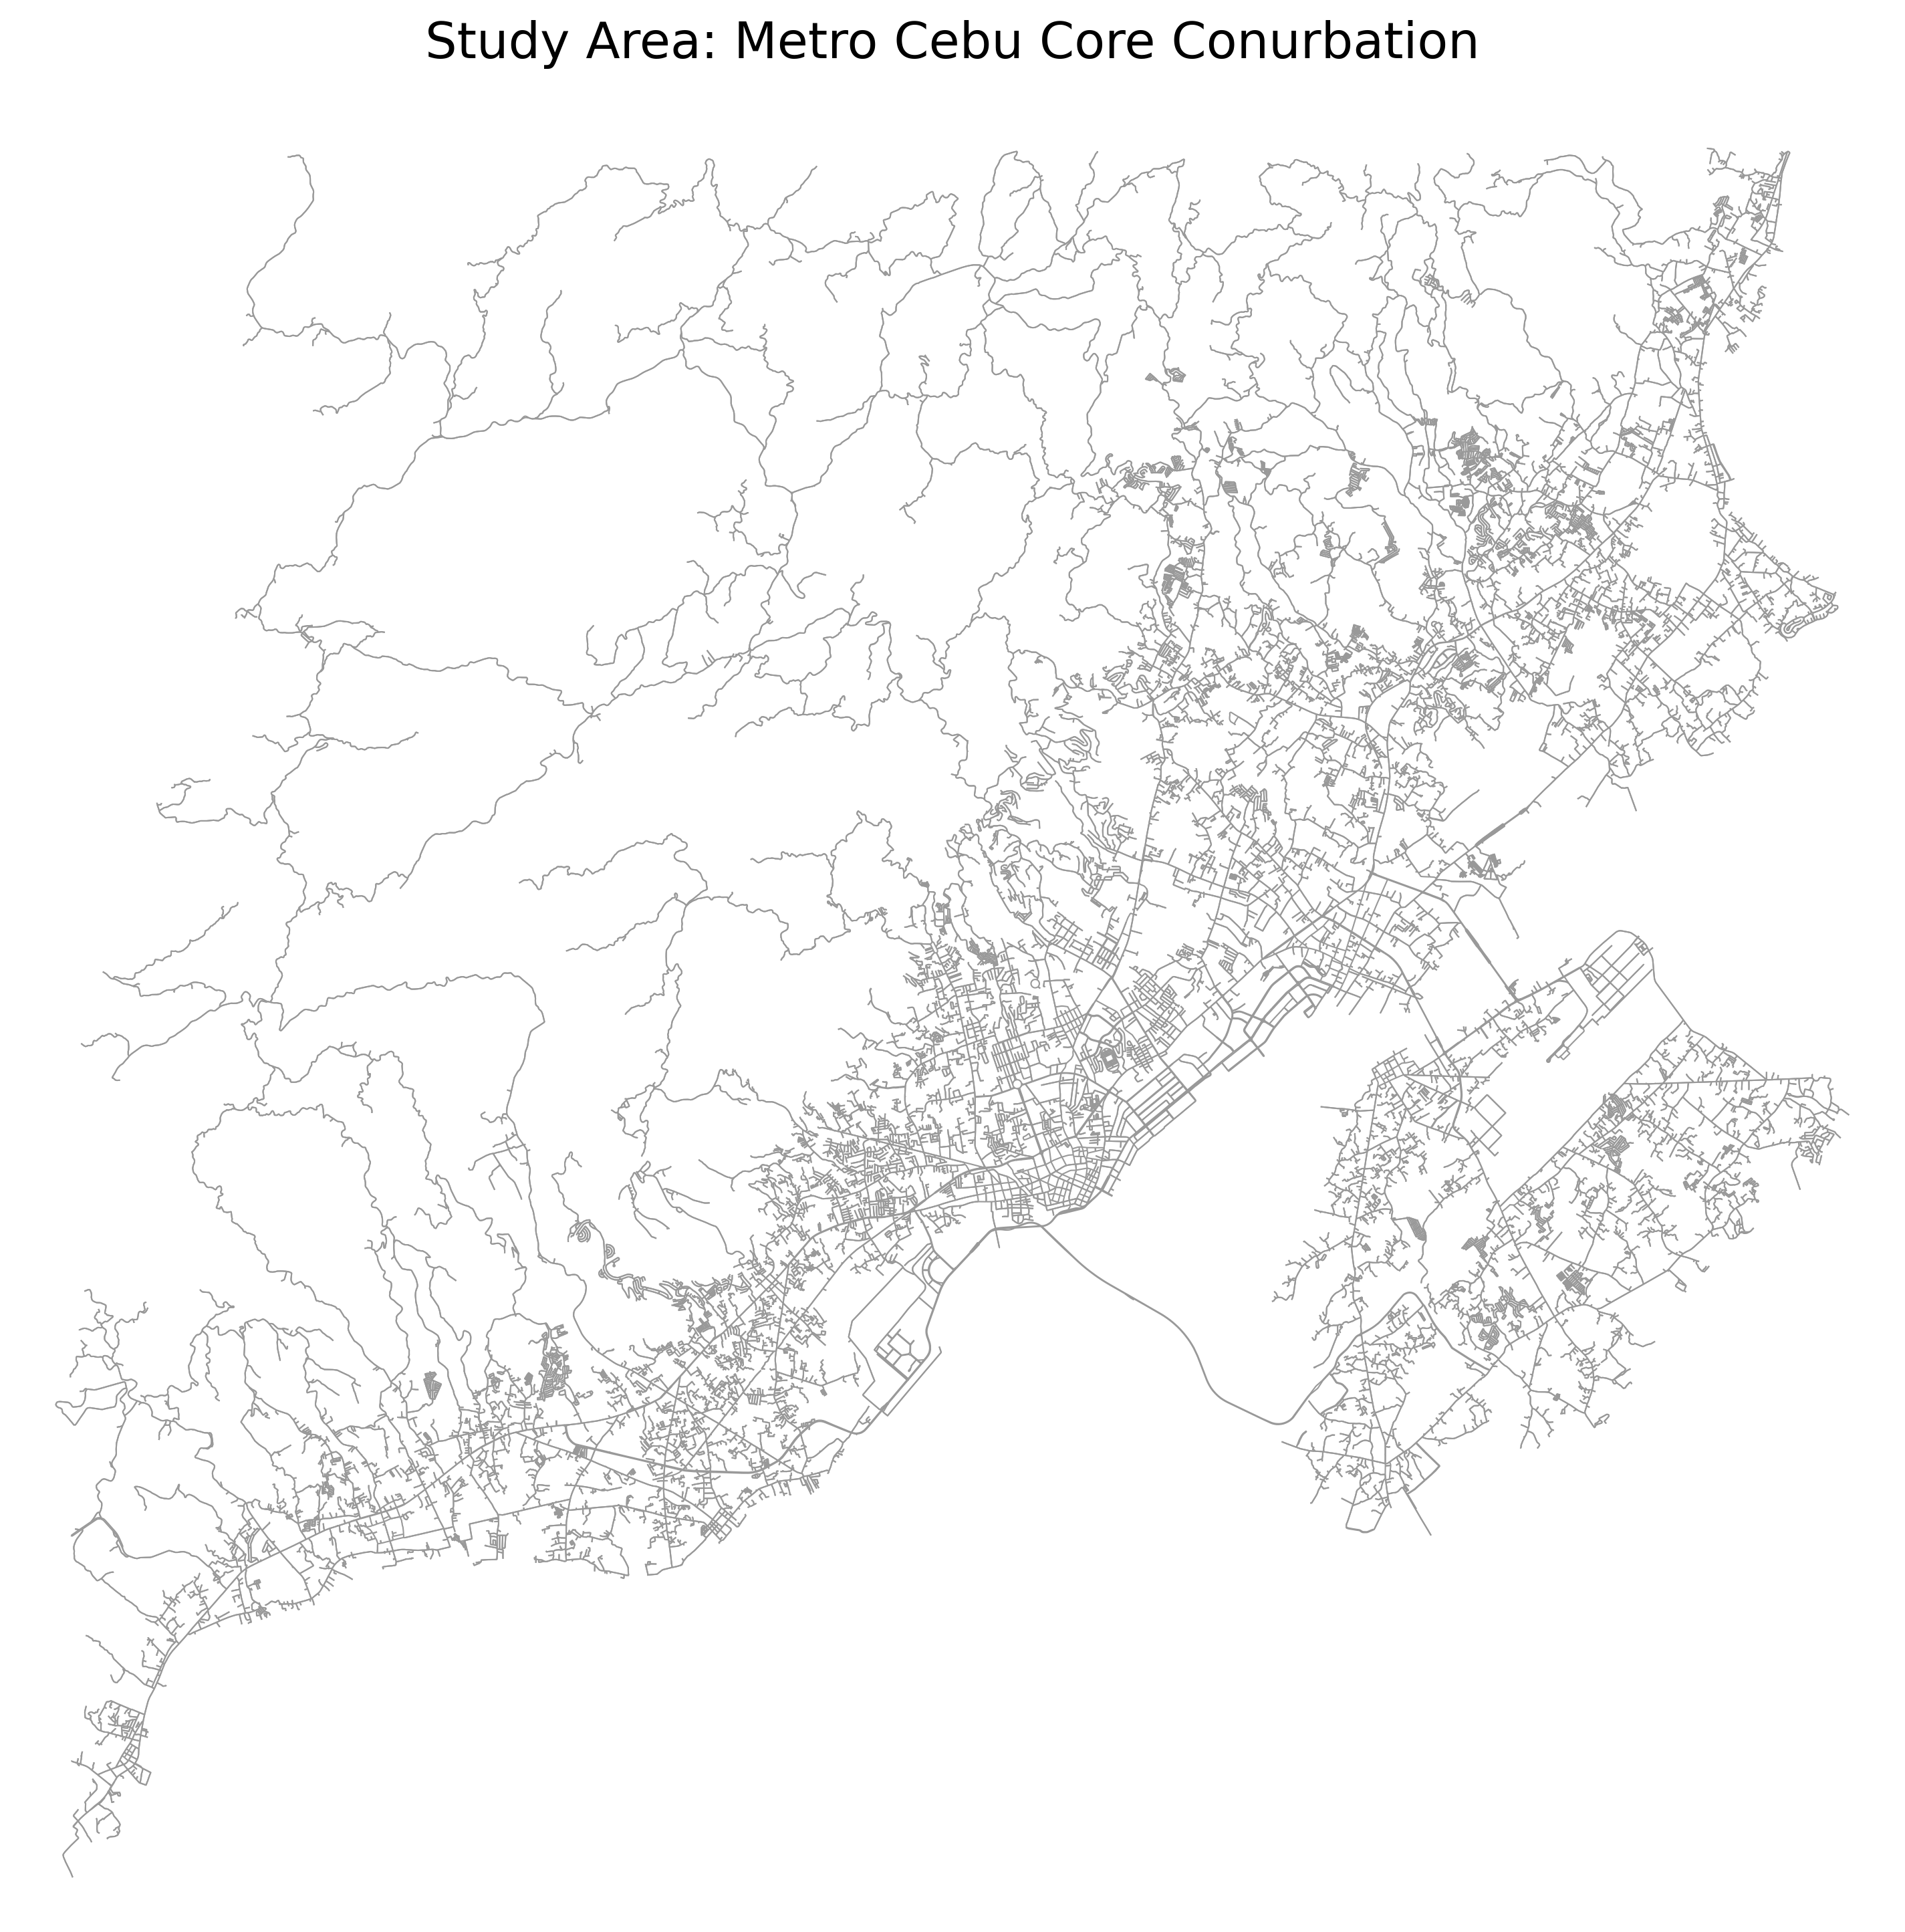
\includegraphics[width=0.90\textwidth]{diagrams/Study-Area-Map.png}
\caption{Metro Cebu Study Area. The six LGUs in the study scope are shown alongside the eight polycentric CBD nodes used for network-distance feature engineering: Cebu Business Park, Mandaue CBD, Mactan CBD, South Road Properties, Talisay Tabunok, Consolacion, Naga City (anchor only), and Mactan-Cebu International Airport.}
\label{fig:study-area}
\end{figure}

The primary data sources include:

The study drew on six data sources covering open-market listings, bank foreclosure records, administrative floor-price benchmarks, BIR zonal values, geospatial APIs, and road network data. Each source is described in detail in Chapter 3, Section 3.2.

The study evaluated three predictive models: \textbf{Hedonic Regression (OLS)}, \textbf{Random Forest}, and \textbf{XGBoost} (see Section 1.6 for rationale). Geospatial features were engineered through geocoding, road-network distance, MCRAI scoring, and spatial lag computation. The canonical ABT preserved the wider market evidence base, but the final fitted model was restricted to the \emph{open\_market} segment so that the deployed output stayed aligned with a market-value use case.

The study produced two applied deliverables: QGIS-ready spatial layers for valuation review and a Streamlit web application combining an open-market residential price surface with property-level prediction and explanation.

\subsubsection{\texorpdfstring{\textbf{Limitations}}{Limitations}}\label{limitations}

\begin{enumerate}
\item \textbf{Open-Market Listing Bias}: The deployed model was fitted on open-market listings rather than verified deed-of-sale transactions. This kept the prediction target aligned with market-facing pricing, but it also meant that seller strategy and asking-price noise remained in the data.
\item \textbf{Unobserved Heterogeneity}: The model cannot capture qualitative features omitted from listings, such as interior finish quality or views, typically assessed during physical inspections.
\item \textbf{Geospatial Approximation}: Addresses are geocoded via Google Maps API, which may introduce minor spatial errors compared to exact lot-parcel shapefiles. Additionally, OSM coverage in peripheral barangays may be less robust than in the urban core.
\item \textbf{Temporal Scope}: The analysis provides a cross-sectional snapshot as of late 2025; it does not capture long-term cyclical real estate trends.
\item \textbf{Geographic Coverage}: The six selected LGUs represent the urban conurbation but exclude the broader municipalities of Cebu Province.
\end{enumerate}

\begin{center}\rule{0.5\linewidth}{0.5pt}\end{center}

\subsection{\texorpdfstring{\textbf{Model Selection Rationale}}{Model Selection Rationale}}\label{model-selection-rationale}

This study employs three complementary models that span the interpretability--accuracy spectrum. This trio has been validated in comparable emerging-market real estate studies \parencite{yacim2018,pai2020}.

\begin{itemize}
\item \textbf{Hedonic Regression (OLS)} serves as the interpretable baseline. It is the established standard in property valuation \parencite{rosen1974}, embedded in both the Philippine Valuation Standards (PVS, 2018) and IVS 2025. OLS produces explicit coefficients for each value driver, directly quantifying their price contribution. We extend it with a spatial lag term to account for autocorrelation among neighboring properties.
\item \textbf{Random Forest} \parencite{breiman2001} addresses the linearity assumption of OLS by capturing non-linear interactions between value drivers---particularly relevant for Metro Cebu housing data, where structural and locational effects are unlikely to remain linear. Its bagging mechanism also provides robustness against outliers.
\item \textbf{XGBoost} \parencite{chen2016} was included as a strong candidate for predictive accuracy: gradient boosting consistently performs well on structured tabular data \parencite{grinsztajn2022} and integrates natively with SHAP \parencite{lundberg2017} to provide property-level explainability, a practical requirement under IVS 2025 transparency standards. The final evaluation in Chapter 7 determines which model best meets the deployment criteria.
\end{itemize}

\subsubsection{\texorpdfstring{\textbf{Why Not Other Models?}}{Why Not Other Models?}}\label{why-not-other-models}

Several alternatives were evaluated but ultimately set aside:

\begin{table}[htbp]
\caption{Models Considered but Not Retained in the Study Design}
\label{tab:chapter1-model-exclusions}
\begin{center}
\begin{tabular}{p{0.23\textwidth} p{0.63\textwidth}}
\toprule
Model & Rationale for Exclusion \\
\midrule
Deep Neural Networks & Require \textgreater{}10,000 labeled samples; our dataset size is insufficient, and global interpretability is sacrificed. \\
Support Vector Regression & Computationally expensive to tune; poor native interpretability; generally weaker than boosting on tabular data. \\
LASSO / Ridge & Constrained by linearity assumptions; effectively subsumed by the OLS baseline for our purposes. \\
\bottomrule
\end{tabular}
\end{center}
\end{table}

\begin{center}\rule{0.5\linewidth}{0.5pt}\end{center}
